\section{Simulation Model Description}

In this section the Arena model is described and explained. The model has been split into two models, firstly the management of the cashiers (main model) and secondly the management of the vehicles (submodel Pumps). The used variables, attributes and schedules will be described as well.

\subsection{Cashier management}
First we describe this model such that it is known what this model does and how it works but not the details how this works. The details will be described after that. In fact what this model does is that it creates five checkouts at the start. These checkouts are the entities which go through the system. When cashiers arrive they are put in a set of available cashiers and the checkouts seize a cashier. When a cashier is seized the checkout opens its associated lanes for 4 hours and after that it is decided if another cashier takes over the checkout or if the checkout closes. If it closes all the vehicles currently in the lane will be served and and then the cashier leaves. If another cashier takes over the checkout the old cashier restocks the supplies and goes home. Just before the cashier finishes its shift a duplicate of the checkout is created, since the old entity of this checkout leaves the system after the shift. The duplicate behaves the same as the old entity and the model continues with still five checkouts. A figure of the complete cashier management model can be found in figure \ref{fig:model-cashier} in appendix \ref{app:modeldescription}.

Now lets discuss the model in more detail with figures. We will handle each different module on the figure. The first part of the model is shown in  figure \ref{fig:createcheckouts}. The first module is $Create \ Checkout$. This module creates at the start of every simulation five checkouts. These checkouts are assigned a number from 1 to 5 in the next module, $Assign \ checkout \ numbers$, so we differentiate the checkouts. After this these five checkouts will remain in $Seize \ Cashier$ until a cashier is available in the model. The model has 12 different resources, each which represents a shift. In every shift it is stated when and for how long cashiers will work. These cashiers are put as resources in the set $Cashiers$, when there are available cashiers in this set a checkout will seize one and continue in the model. 
The last two modules are the $OnChange$ and $Assign \ Duplicate \ Checkoutnumber$ which do the same as the first two modules, only now for duplicate checkout entities. The $OnChange$ is triggered when a cashier is almost finished working his shift as mentioned above.

\begin{figure}[h!]
\begin{center}
	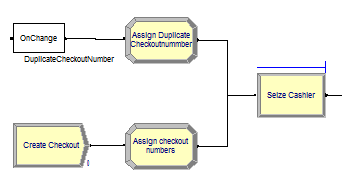
\includegraphics[scale=1]{images/model-description/checkout-creation.PNG}
	\caption{Modeling of the creation of checkouts.}
	\label{fig:createcheckouts}
\end{center}
\end{figure}

The second part of the model is shown in figure \ref{fig:seizeandopen}. When a cashier was seized the checkout moved on to $Active \ Cashiers \ smaller \ than \ 5?$. In this module it is checked whether the shift of the original checkout is finished before the duplicate checkout may move on. If this is not checked it is theoretically possible that both the original checkout and the duplicate checkout are manned. After this module all the associated lanes of the checkout are opened in $Open \ checkout$.

\begin{figure}[h!]
\begin{center}
	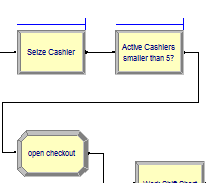
\includegraphics[scale=1]{images/model-description/seize-and-open.PNG}
	\caption{Modeling of the cashier seizing and checkout opening.}
	\label{fig:seizeandopen}
\end{center}
\end{figure}

The next part of the model is shown in figure \ref{fig:workshift}. After that the checkout has opened its associated lanes we first check whether it's a 2 hour or a 4 hour shift. This is necessary because at the start of the simulation (0:00) cashiers from shift 12 are already working and they have only 2 hours left. So these cashiers will go to module $Work \ Shift \ Short$ where a delay of 1 hour and 50 minutes will represent working a shift for the same amount of time. All the other cashiers will go to $Work \ Shift$ where they work for 3 hours and 50 minutes. After these delays the cashiers checkouts reach the module $Trigger \ OnChange$. In this module we trigger the $OnChange$ module mentioned before so that the checkout in this module will be duplicated. Next the cashiers work their remaining 10 minutes in $Work \ Remaining \ Shift$. When the cashier is completely done with his regular shift we decrease the number of active cashiers so that possibly stuck duplicate checkout can continue from the $Active \ Cashiers \ smaller \ than \ 5?$ module we saw before.

\begin{figure}[]
\begin{center}
	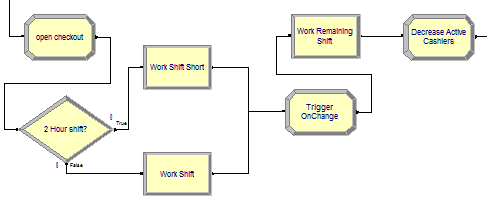
\includegraphics[scale=1]{images/model-description/work-shift.PNG}
	\caption{Modeling of the delay for the cashier working his/her shift.}
	\label{fig:workshift}
\end{center}
\end{figure}

After the regular shift, we have to determine what will happen to the lanes and the cashier. Does he close the lanes and continue working at the checkout till the lanes are empty? Or does another cashier take over and can he go over to restocking the supplies? This is checked in the blocks displayed in figure \ref{fig:determinetakeover}. As you can see, the check whether someone takes over is split into two checks. This is due to a technicality issue: we have a global 1D array with 5 rows. Every row contains a time stamp. This time stamp represents the latest shift which started for that checkout. So in the upper right module $Pump \ Stays \ Open$ we check if the time stamp in the associated row in the array is newer than the expression "TNOW - 3.5", which means is the time stamp less than 3,5 hours old. If not the time stamp is the same as when the shift of the current cashier started and therefore we know the cashier has to close the lanes. If the time stamp is newer it means that another cashier is waiting to take over the shift. The technical problem we have is that for the first 3,5 hours we cannot use this expression, because it will always evaluate to true since there are no negative time stamps. Since shifts only start at whole hours we check if there has past more than 3 hours since the start of the simulation. In the bottom left $Pump \ stays \ Open$ module we just check if the new time stamp is larger or equal to 2, since that is the only shift of cashiers which can take over a checkout before we reach TNOW = 3. 

\begin{figure}[]
\begin{center}
	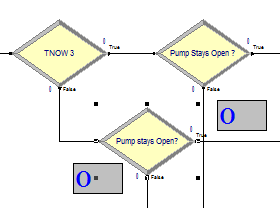
\includegraphics[scale=1]{images/model-description/determine-takeover.PNG}
	\caption{Modeling of the check whether a checkout is taken over.}
	\label{fig:determinetakeover}
\end{center}
\end{figure}

The last part of the cashier management is rather straightforward (figure \ref{closerestockandrelease}): based on the previous decision, the checkout is closed after which the cashier works until the lane and checkout queue are both empty after which he restocks the supplies if less than 10 minutes have passed since the checkout was closed (which is calculated by setting a variable to the current time upon closing and comparing it to current time after the queue is emptied). Or the checkout does not close and the cashier immediately restocks the supplies.
After this the cashier is released and the checkout entity will be disposed.

\begin{figure}[]
\begin{center}
	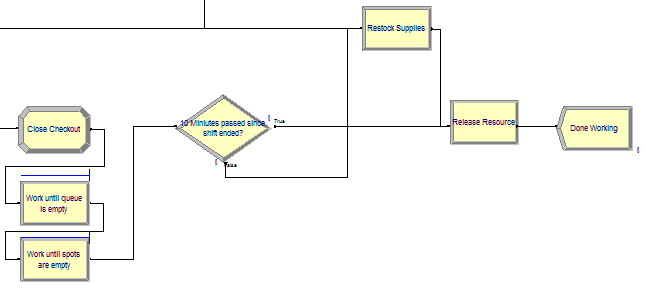
\includegraphics[scale=1]{images/model-description/close-restock-release.PNG}
	\caption{Modeling of the check whether a checkout is taken over.}
	\label{fig:closerestockandrelease}
\end{center}
\end{figure}